% This is "sig-alternate.tex" V2.0 May 2012
% This file should be compiled with V2.5 of "sig-alternate.cls" May 2012
%
% This example file demonstrates the use of the 'sig-alternate.cls'
% V2.5 LaTeX2e document class file. It is for those submitting
% articles to ACM Conference Proceedings WHO DO NOT WISH TO
% STRICTLY ADHERE TO THE SIGS (PUBS-BOARD-ENDORSED) STYLE.
% The 'sig-alternate.cls' file will produce a similar-looking,
% albeit, 'tighter' paper resulting in, invariably, fewer pages.
%
% ----------------------------------------------------------------------------------------------------------------
% This .tex file (and associated .cls V2.5) produces:
%       1) The Permission Statement
%       2) The Conference (location) Info information
%       3) The Copyright Line with ACM data
%       4) NO page numbers
%
% as against the acm_proc_article-sp.cls file which
% DOES NOT produce 1) thru' 3) above.
%
% Using 'sig-alternate.cls' you have control, however, from within
% the source .tex file, over both the CopyrightYear
% (defaulted to 200X) and the ACM Copyright Data
% (defaulted to X-XXXXX-XX-X/XX/XX).
% e.g.
% \CopyrightYear{2007} will cause 2007 to appear in the copyright line.
% \crdata{0-12345-67-8/90/12} will cause 0-12345-67-8/90/12 to appear in the copyright line.
%
% ---------------------------------------------------------------------------------------------------------------
% This .tex source is an example which *does* use
% the .bib file (from which the .bbl file % is produced).
% REMEMBER HOWEVER: After having produced the .bbl file,
% and prior to final submission, you *NEED* to 'insert'
% your .bbl file into your source .tex file so as to provide
% ONE 'self-contained' source file.
%
% ================= IF YOU HAVE QUESTIONS =======================
% Questions regarding the SIGS styles, SIGS policies and
% procedures, Conferences etc. should be sent to
% Adrienne Griscti (griscti@acm.org)
%
% Technical questions _only_ to
% Gerald Murray (murray@hq.acm.org)
% ===============================================================
%
% For tracking purposes - this is V2.0 - May 2012

\documentclass{sig-alternate}

\usepackage{listings}

\begin{document}
%
% --- Author Metadata here ---
\conferenceinfo{Foss4g Europe}{'14 Bremen, Germany}
%\CopyrightYear{2007} % Allows default copyright year (20XX) to be over-ridden - IF NEED BE.
%\crdata{0-12345-67-8/90/01}  % Allows default copyright data (0-89791-88-6/97/05) to be over-ridden - IF NEED BE.
% --- End of Author Metadata ---

\title{Open Source pedestrian routing service with OpenStreetMap Data for blind people
\titlenote{(Produces the permission block, and
copyright information). For use with
SIG-ALTERNATE.CLS. Supported by ACM.}}
\subtitle{PgRouting, OpenTripPlanner and OpenSourceRoutingMaschine
\titlenote{A full version of this paper is available as
\textit{Author's Guide to Preparing ACM SIG Proceedings Using
\LaTeX$2_\epsilon$\ and BibTeX} at
\texttt{www.acm.org/eaddress.htm}}}
%
% You need the command \numberofauthors to handle the 'placement
% and alignment' of the authors beneath the title.
%
% For aesthetic reasons, we recommend 'three authors at a time'
% i.e. three 'name/affiliation blocks' be placed beneath the title.
%
% NOTE: You are NOT restricted in how many 'rows' of
% "name/affiliations" may appear. We just ask that you restrict
% the number of 'columns' to three.
%
% Because of the available 'opening page real-estate'
% we ask you to refrain from putting more than six authors
% (two rows with three columns) beneath the article title.
% More than six makes the first-page appear very cluttered indeed.
%
% Use the \alignauthor commands to handle the names
% and affiliations for an 'aesthetic maximum' of six authors.
% Add names, affiliations, addresses for
% the seventh etc. author(s) as the argument for the
% \additionalauthors command.
% These 'additional authors' will be output/set for you
% without further effort on your part as the last section in
% the body of your article BEFORE References or any Appendices.

\numberofauthors{3} %  in this sample file, there are a *total*
% of EIGHT authors. SIX appear on the 'first-page' (for formatting
% reasons) and the remaining two appear in the \additionalauthors section.
%
\author{
% You can go ahead and credit any number of authors here,
% e.g. one 'row of three' or two rows (consisting of one row of three
% and a second row of one, two or three).
%
% The command \alignauthor (no curly braces needed) should
% precede each author name, affiliation/snail-mail address and
% e-mail address. Additionally, tag each line of
% affiliation/address with \affaddr, and tag the
% e-mail address with \email.
%
% 1st. author
\alignauthor Markus Dornhofer\\
       \affaddr{FH JOANNEUM}\\
       \affaddr{Energy and Transportation}\\
       \affaddr{Kapfenberg - Austria}\\
       \email{markus.dornhofer @fh-joanneum.at}
% 5th. author
\alignauthor Werner Bischof\\
       \affaddr{FH JOANNEUM}\\
       \affaddr{Energy and Transportation}\\
       \affaddr{Kapfenberg - Austria}\\
       \email{werner.bischof @fh-joanneum.at}
% 6th. author
\alignauthor Elmar Krajnc\\
       \affaddr{FH JOANNEUM}\\
       \affaddr{Internet Technology}\\
       \affaddr{Kapfenberg - Austria}\\
       \email{elmar.krajnc @fh-joanneum.at}
}


\maketitle




\begin{abstract}
This paper provides a sample of a \LaTeX\ document which conforms,
somewhat loosely, to the formatting guidelines for
ACM SIG Proceedings. It is an {\em alternate} style which produces
a {\em tighter-looking} paper and was designed in response to
concerns expressed, by authors, over page-budgets.
It complements the document \textit{Author's (Alternate) Guide to
Preparing ACM SIG Proceedings Using \LaTeX$2_\epsilon$\ and Bib\TeX}.
This source file has been written with the intention of being
compiled under \LaTeX$2_\epsilon$\ and BibTeX.

The developers have tried to include every imaginable sort
of ``bells and whistles", such as a subtitle, footnotes on
title, subtitle and authors, as well as in the text, and
every optional component (e.g. Acknowledgments, Additional
Authors, Appendices), not to mention examples of
equations, theorems, tables and figures.

To make best use of this sample document, run it through \LaTeX\
and BibTeX, and compare this source code with the printed
output produced by the dvi file. A compiled PDF version
is available on the web page to help you with the
`look and feel'.
\end{abstract}

% A category with the (minimum) three required fields
\category{H.4}{Information Systems Applications}{Miscellaneous}
%A category including the fourth, optional field follows...
\category{D.2.8}{Software Engineering}{Metrics}[complexity measures, performance measures]

\terms{Theory}

\keywords{ACM proceedings, \LaTeX, text tagging}
\section{Introduction}
For visually impaired and blind people the fastest or the shortest route is not the important fact, they prefer the safest route from a start point to an end point. There are some navigation systems for blind users available on the market, but no system make an highly uses of additional data for blind users. 
OpenStreetMap contains very useful information for visually impaired and blind people. It make it possible to find a safe route from a start point to an end point, which includes acoustical traffic signals and safe sidewalks.Also additional information can improve the navigation. If the user is told that the building is on the right hand side, he/she can verify the information and improve the positioning. Or a warning can occur in front of a waste basket or a traffic sign in an critical position (i.e closed to the head). 
 
There are many Open Source Routing Systems available today. Many of them focus on car navigation, bicycle navigation and pedestrian navigation. Some of them even include multimodal routing in combination with public transportation systems. In this paper a comparison between different open source routing engines (pgrouting,opentripplanner and open source routing machine) should be made. And how the transfer the technology from car navigation to pedestrian navigation can be done. 
\section{User Requirements}
navigation device should be a smartphone with no additional device
The user interface should be barrier free [Elmar Paper]
How to enter a target address on a smartphone
Less disturbance with the environment
during navigation free hands for the blindman stick an additional stuff
The navigation App should also work in the background

\section{Related Work}

Loadstone GPS:
The pioneer in free GPS navigation software is Loadstone GPS\cite{loadstone}. It is running on Symbinan mobile phones and uses an external bluetooth GPS receiver. The product is very popular in the community of blind and visually impaired people.

Blindsquare:
Blindsquare\cite{blindsquare} is an Iphone App and uses point of interest information from foursquare and OpenStreetMap. The actual price is about US dollar 24. 

OSMAnd Maps and Navigation:

Weyrer (FH K\"{a}rnten): 
Timothy Weyrer\cite{weyrer} wrote a master thesis about intermodal door-to-door application for people with disabilities on the carinthia university of applied sciences.

Sven Leitinger (SR):
Sven Leitinger\cite{sven:osm} from Salzburg Research wrote a guideline to enhance the OSM Data with blind related attibutes. He explained most of the OSM tag, which are useful for blind people. The work focus on existing OSM tags and are not creating new features. But no prioritisation of OSM tag had been made. 

\section{Project Ways4all}


\section{OSM Related}
\begin{description}
  \item tactile
  \item surface
  \item footway type
  \item crossing
  \item kerb
\end{description}

\section{Routing}
Five requirements\cite{weyrer}:
\begin{description}
  \item A procedure to set start point and end point
  \item A connected network (routing graph), on which the routing can be performed
  \item An algorithm that computes the route between start point and end point
  \item The inclusion of user requirements in the route computation and selection
  \item The presentation of the results to the use
\end{description}


\section{Comparison between different routing tools (in context to blind persons)}

What information is in the routing graph? What streets are prefered by blind persons? What solution is the best?
The Webfrontend is not required for the blind users, but it is important for the developer. It is easy to test different routes and it gives you a good impression about the speed of the routing service.

\begin{figure}
\centering
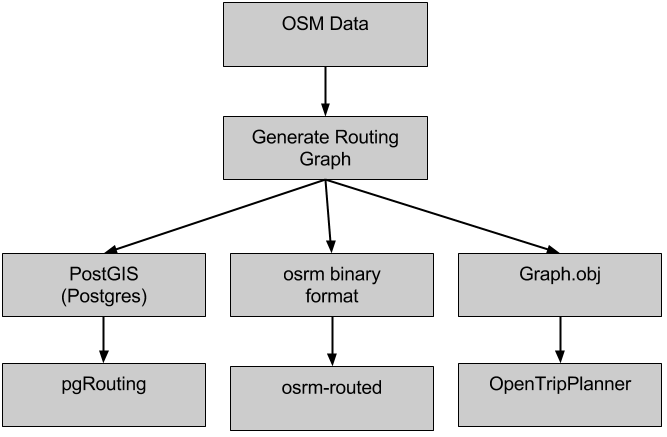
\includegraphics[width=3in]{Overview2.png}
\caption{Overview}
\end{figure}

\subsection{pgrouting\cite{pgrouting}}
Database, many differnent shortest path algorithms, no turn instructions, easy to get geojson track with server side programming languarge (i.e. PHP). no Web-Frontend


\lstinputlisting[language=Xml,basicstyle=\footnotesize,breaklines=true,frame=lines,caption={osm2pgrouting}]{mapconfig_for_cars.xml}

\subsection{OpenTripPlaner}
 
The OpenTripPlaner servlet runs on any standards-compliant Java web server. It is a complete bundle with includes a REST API and a Webfrontend. The Webfrontend let you set an start and end point and with button a route can be requested. Drag and Drop the markers as with the OSRM Webfrontend is not possible. The route request takes much more time as with the OSRM routing service. For other Applications like Smartphone Apps there is a well dokumentated REST API, where a route can be requested with many parameters. One routing process can handle multiple profiles (i.e. Walking, Bicycle and Car) and intermodal transportation. GTFS (General Transit Feed Specification) format from Google is used to query the timetables from public transportation companies. 

\begin{description}
  \item[+] includes public transportation ( GTFS)
  \item[+] intermodal (i.e. walk and public transportation) transportaion
  \item[+] well documented REST API
  \item[+] seperated JAVA web-apps (Webfrontend and Routing Service)
  \item[+] less dependencies (any standards-compliant Java web server)
  \item[+] multiple profies (Bike, walk, transit) handled by a single routing process
  \item[+] walk speed selectable
  \item[+] safety options in the configure file available
  \item[+] easy to configuration with xml file
  \item[+] Logging and Debugging 
  \item[-] slow route calculation
  \item[-] need much resources to build routing graph   
\end{description} 
 
\begin{figure}
\centering
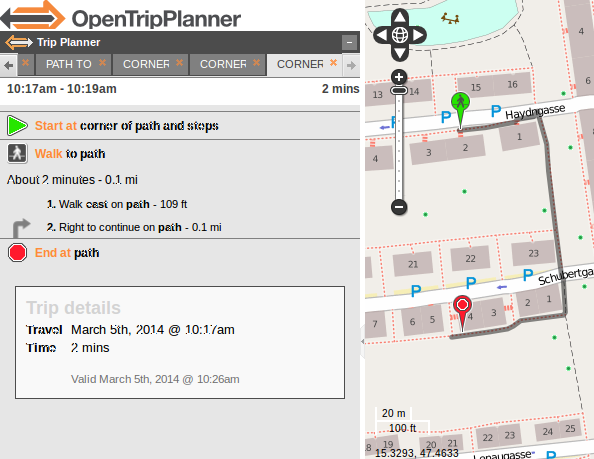
\includegraphics[width=3in]{otp-ss.png}
\caption{Overview}
\end{figure}
 
 The graph builder is controlled by an XML configuration. For big regions (i.e. the Country Austria) a lot of RAM is needed. OpenTripPlanner is intended for small and medium geographic areas, but with huge amount of RAM also big areas are possible. The safety parameter was invented for bicycles. There can be a notification, if the osm key surface  has a specific value (i.e. 'Caution: muddy!'). The safe value 1 is default. Very safe streets can have a value below 1 and for dangerous streets can be give a value more than 1. The distance of a street segment will be multiplied with the safe value. I.e. A ten times more dangerous street will have the the length of the street times 10. \\
 With a permission key all transportation types (i.e. Pedestrian, Bicycle, ..) can be put on a white list. So street segment can be accessed by this type of transportation. \\
 It should be possible to convert the bicycle safety features to pedestrian safety features.
 
\lstinputlisting[language=Xml,basicstyle=\footnotesize,breaklines=true,frame=lines,caption={GraphBuilder OTP}]{otp-config.xml}


\subsection{OSRM}

\begin{description}
\item[+]very fast, 
\item[+]generates the graph on the settings in a profile.lua file
\item[+]lua configuration for routing graph (lua script language ), 
\item[+]shortest path calculation contraction hierarchies, faster then dijskta algorithm
\item[+]+blacklist of street, which should not be used
\item[+]delivers gpx track or turn instruction list in json,
\item[+]nice Web frontend, supports multiple targets,
\item[-] no safety properties, influence the route with different speed parameters, a safe street get a high speed value
\end{description}

\begin{figure}
\centering
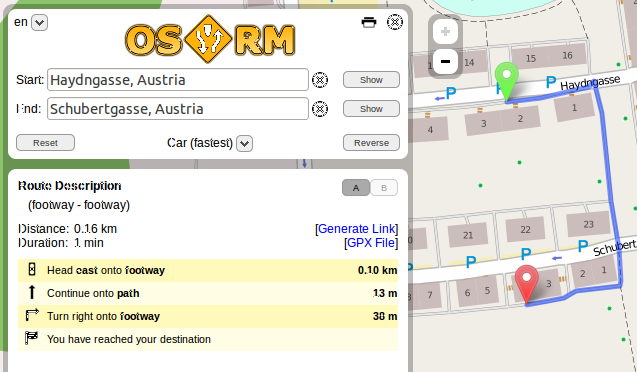
\includegraphics[width=3in]{osrm-ss.png}
\caption{Overview}
\end{figure}

C++,No turn instruction if the road name stays the same. Made for cars


\begin{table}
\centering
\caption{Example Routing List}
\begin{tabular}{|c|c|c|c|c|} \hline
No&Turn Angle&Road Name/Type&Distance&Heading\\ \hline
4&282&Werk-VI-Strasse&250m&NW\\ \hline
12&14&Path&24m&SW\\ \hline
\end{tabular}
\end{table}

\lstinputlisting[basicstyle=\footnotesize,breaklines=true,frame=lines,caption={osrm}]{foot-osrm.lua}

\section{System Design}
The system was designed as Server/Client Infrastructure. The network graph is held on the server and the routing calculation is also done on the server.  The client ask for the best route with a start point and an destination. Even multiple destination can be handled by the server. Then the server replies with a Json formated file. The json file contains the gpx Track and turn instructions on specific track points. The turn instructions contain the turn angle, the street name or road type, the distance to the next turn instruction and the heading information (i.e. North West) 

A network connection is needed for every route request. 

\section{First Results and Tests}
The Android App development started in the same time as the comparison between the routing machines. It was clear that the App request a route with a start and a stop position and the server replies with a well structured (i.e. XML or JSON) format. \\
The user interface and the navigation are much more important on the smartphone. The routing server should be replaceable. 
By the way a OSRM Routing Service was chosen for the first test. On the app side a target position can be selected from a list and the actual position was used as start position. After the routing response is displayed in a new list (figure ~\ref{fig:app}). \\
The user can explore the whole trip on the screen. Turn instruction by turn instruction. The distance to the next turn instruction is spoken periodically. If the proximity of the crossing point is reached the turn instruction was told. \\

 

\begin{figure}
\centering
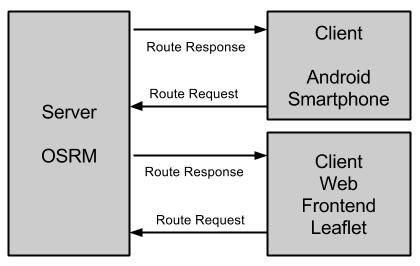
\includegraphics[width=3in]{System-Design2.png}
\caption{System Design}
\end{figure}

\begin{figure}
\centering
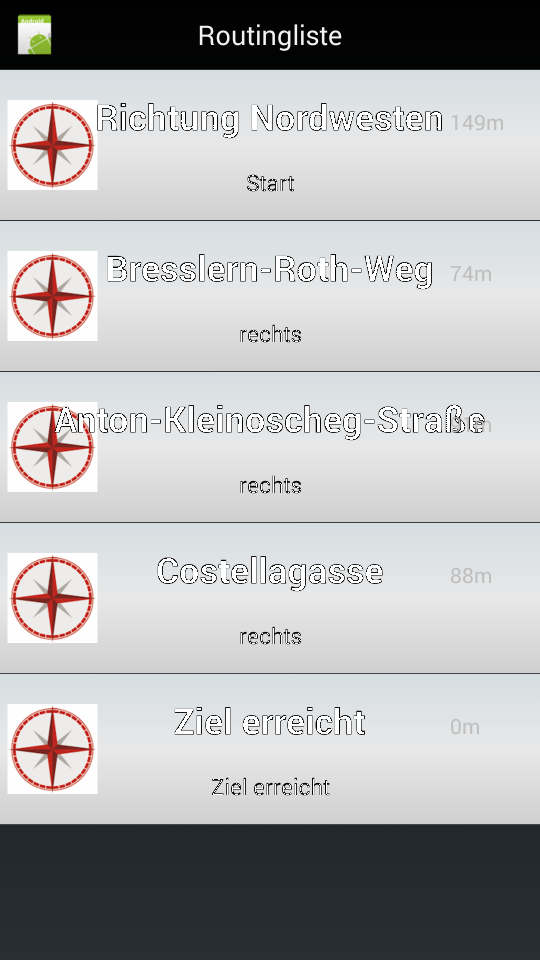
\includegraphics[width=3in]{App2.png}
\caption{Android App}
\label{fig:app}
\end{figure}


\section{Conclusion}



\section{Future work}
The first version was just a prove of concept. The main focus was on the user interface and on a stable server and client communication. The navigation has to be  improved a lot. There has to be a mode where blind people can follow a track in a park without much kerbs. Also a module is needed to get information about the near environment (i.e. Position of the road or building. This information could not be found in the route. There have to be turn instructions where the road stays the same, but makes a curve (i.e. priority roads). \\
Side walks and Streets are closed to each other. It is important that the starting point do not snap to the Street in front the Side walk. \\
And an Evaluation of the priority of footways has to be done. 


\section{Acknowledgements}
The overall project manager is the University of Applied Sciences FH-JOANNEUM in Kapfenberg, Austria. One focus of the project ways4all is to support visually impaired and blind people in their daily lives with the help of usual smartphones. Additional equipment is a no goal of the project. One module focus on indoor and outdoor navigation. \\
Project participants are: Wiener Linien, OEBB and four blind and handicapped organisations. The project is subsidized by the Austrian Federal Ministry
for Transport, Innovation and Technology (BMVIT) and the
Austrian Research Promotion Agency (FFG).

%
% The following two commands are all you need in the
% initial runs of your .tex file to
% produce the bibliography for the citations in your paper.
\bibliographystyle{abbrv}
\bibliography{sigproc}  % sigproc.bib is the name of the Bibliography in this case
% You must have a proper ".bib" file
%  and remember to run:
% latex bibtex latex latex
% to resolve all references
%
% ACM needs 'a single self-contained file'!
%
%APPENDICES are optional
%\balancecolumns

\end{document}
